Experiments in the development set were carried out using 4-Fold Cross Validation. Models
were trained using data from three folds and tested on the remaining one, rotating the
procedure four times over the four partitions. There were no common speakers across any of
the partitions. When reporting results for a given system, the errors obtained for each of the
four folds are pooled to obtain averaged performance results on the development set.

Additionally, a \textit{heldout} set with the same number of instances of each of the folds
in the \textit{development} set
was kept separately to test the final models. There were also no common speakers between
the \textit{heldout} set and any of the folds of the development set. When reporting results
for a given system using the heldout data, the errors are obtained in a straightforward way
by testing the model trained on the development set against the heldout data.

In all the experiments, an individual system is trained for each different phoneme.

\section{Baseline Experiments}

The current work uses the same database used in \cite{main} with the exception that
data is split differently:
In \cite{main}, a four-way jackknifing procedure containing all the instances is used to train
and test the models, while in the current work a heldout set was kept separately of the development
set. The number of Gaussian Mixtures composing each GMM is proportional to the number of
training instances for that phone. In \cite{main}, a proportion of 1/25 computed
beforehand over the total number of instances was used. In the current work, only 60\% of the
total instances for a given phoneme is used to train each model, so the proportion of Mixture
Components per number of instances was set to 1/15 to preserve the number of Gaussians of each
model.

The initial experiments were carried out in order to replicate the results obtained in \cite{main} (task that should be possible because of using the same database).
These systems could then be used as baselines and as starting points for the next systems.
In this previous work three different systems are compared:

\begin{enumerate}
	\item Independenty Trained GMMs
	\item Adapted GMMs
	\item SVMs trained on supervectors
\end{enumerate}

Results presented in \cite{main} had shown that the adaptation of the class-independent GMM produced
an overall weighted EER relative reduction of 3.5\% relative to the results
obtained with independently trained GMMs.

Two initialization approaches to be performed before training the GMMs
were explored in the current work: \textit{KMeans} and \textit{Agglomerative Clustering}. The
objective was to see if additional gain could be obtain by performing an additional initialization
before training the GMMs. Both approaches were tested in the development set producing similar
results. \textit{Agglomerative Clustering}, however, requires $O(n^{3})$ steps to be computed
(where $n$ is equal to the number of instances), making it very impractical as an initialization
step. For both reasons, \textit{KMeans} was chosen as the representative initialization method.

Results of the Adapted GMM initialized with KMeans experiment performed in the development set
generated a 3\% relative reduction of the overall weighted EER compared with results of
Independently Trained GMMs initialized with KMeans.
These results, as it was
expected, are strongly correlated with the results obtained in \cite{main} and
thus determining a succesful replication of the initial experiment. Similar results were obtained
when comparing the Adapted GMMs with the Independently Trained GMMs but using
\textit{Agglomerative Clustering} initialization.

\subsection{GMM Adapt K-Means vs Supervectors}

The next step was to compare the Adapted GMMs systems with the SVMs trained on supervectors.
Results presented in \cite{main} shown that the SVMs systems produced an overall weighted EER
relative reduction of 1.3\% with respect to the Adapted GMMs.

Below is shown the comparison between the results obtained with the Adapted GMMs initialized
with KMeans and the results obtained with the SVMs system in the development set.
The UBM-GMMs used to generate the
supervector features for the SVM are trained using no initialization (such as KMeans) because
it leads to better results.

The results are sorted in descending order according to their Kappa Coefficient.
It seems to be some correlation between the phonemes with high kappa and those who achieved
the best results. This seems reasonable, because it may exist clearer differences
between correctly and mispronounced
utterances of the phonemes that produced better agreement over the transcribers.
These differences may lead the classifiers to perform better.
Among the eight phonemes with higher Kappa values (K $>$ 0.4, which implies moderate agreement):
/$\beta$/, /$\delta$/, /$\gamma$/, /b/, /w/, /m/, /i/, /s/, only /s/ exceeds an EER of 0.3.
Results show that the SVMs system produced an overall weighted EER relative reduction of 2.5\% with
respect to the Adapted GMMs with K-Means initialization, which is in line with the results obtained
in \cite{main}.

\begin{figure}[H]
	\centering
	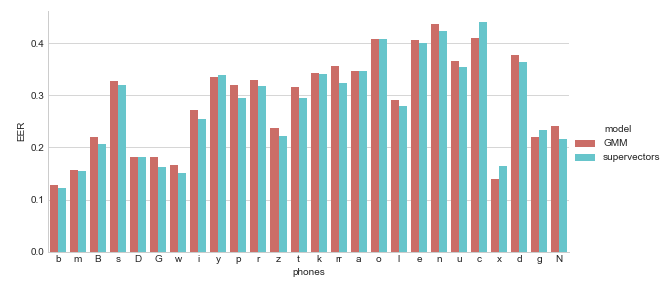
\includegraphics[width=0.8\textwidth]{files/figures/results/gmm-vs-supervectors/gmm-vs-supervectors-dev.png}
	\caption{Comparison of EER between LLR from Adapted GMMs with K-Means initialization
	and SVM trained on Supervectors for all phones in the development set, sorted
	descendently by Kappa values.}
	\label{fig:gmmSupervectorsDev}
\end{figure}

The same experiment was carried out in the heldout set leading to the results shown below.
Both models were trained using all the instances in the development set.
Both systems had a very similar performance for each phoneme compared with the results obtained
in the development set, from which one can deduce that both classifiers generalize well to
unobserved data. This time, however, it was the Adapted GMM with K-Means initialization
which produced an overall weighted EER relative reduction of 0.8\% with respect to the SVMs
trained on supervectors. Even though the expected result would have been that the SVM performed
slightly better than the GMM as in \cite{main} and as it occurred in the development set,
the degradation is less than 1\% so it is still a reasonable result. In all the experiments
carried out to compare the SVMs trained on supervectors and the Adapted GMMs, both classifiers
shown a very similar performance on each phoneme.

After the successful replication of the initial experiments, a validated SVM model based on
supervectors was obtained. This classifier is used as baseline and starting point for
the next experiments,
whose objective is to analyse if an aditional gain in the performance could be achieved by
combining the supervectors features with features that carry temporal information.

\begin{figure}[H]
	\centering
	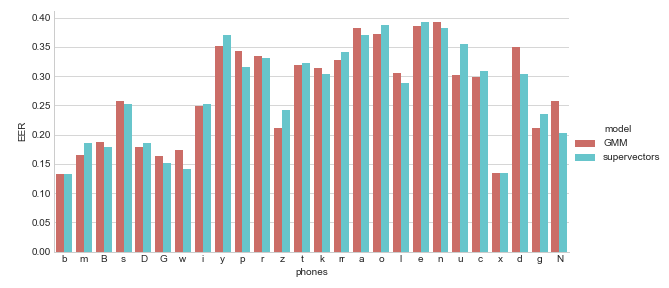
\includegraphics[width=0.8\textwidth]{files/figures/results/gmm-vs-supervectors/gmm-vs-supervectors-heldout.png}
	\caption{Comparison of EER between LLR from Adapted GMMs with K-Means initialization
	and SVM trained on Supervectors for all phones in the heldout set, sorted descendently
	by Kappa values.}
	\label{fig:gmmSupervectorsTest}
\end{figure}

\section{Tunning Experiments}

Tunning experiments are carried out in order to compare both alternative
dynamic features that capture the temporal dependencies on each instance. These features are
used as training instances of an SVM classifier.

Features are first analysed in isolation to determine the best possible configuration for
each technique. After that, the features generated with these configurations are combined with
the supervectors and compared to each other.

Tunning is again performed in the deveopment set using 4-Fold Cross Validation. Results are
calculated only for the phonemes with high Kappa values taking the average of all the values.
Only these phonemes are considered in the process because they are the most reliable ones.

The optimal parameters to be obtained at this point: mainly the number of coefficients to
be used of both Legendre and DCT, are shared by all the phonemes. This helps to keep
the models simple by reducing the number of phone-dependent configuration parameters.

\subsection{Legendre Best System}

Tunning the best Legendre configuration involves the analysis of three different parameters:

\begin{itemize}
	\item Time axis normalization between -1 and 1
	\item Inclusion of duration
	\item Lasso-Regression normalization
\end{itemize}

The objective of the Legendre tunning experiments is to find the optimum degree of the Legendre
Polynomials along with the decision of normalizing or not the time axis and applying or not
Lasso Regularization over the coefficients. Degree was varied between 0 and 6,
because polynomials with
higher degrees run the risk of overfit to training instances by modeling very specific not
generalizable details.


\begin{figure}[H]
	\centering
	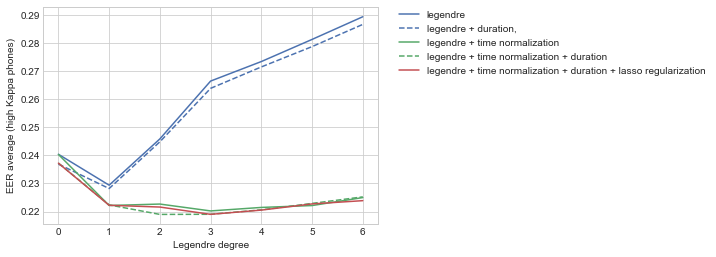
\includegraphics[width=1.0\textwidth]{files/figures/results/legendre-dct/legendre-tunning.png}
	\caption{EER average over phonemes with high Kappa for different
	degrees of Legendre Polynomials in
	the training set. Additional configurations are also studied along with the degree and
	represented by different curves: time normalization, appending the duration and applying
	Lasso Regression}
	\label{fig:legendreTunning}
\end{figure}

Time normalization before approximating the
MFCCs turned out to be an essential property for the Legendre Polynomials, evidenced by a
considerable reduction of the EER average (gap between the blue and green curves). At the same
time, appending the duration to the features produced a slight improvement in the performance.
Lasso Regularization, however, does not contribute to reduce the average EER.
Results show that the optimal configuration is to model the dynamics of the temporal dependencies
using Legendre Polynomials of degree 2, normalizing the time axis and appending the duration of the
phone utterance to the features (green dotted line).

\subsection{DCT Best System and Comparison Between Features}

Analogous to Legendre, the objective of the DCT tunning experiments is to find the optimum
number of coefficients of DCT to approximate the dynamics of the temporal dependencies.
In the DCT case, the only additional parameter to be determined is whether or not appending the
duration to the DCT coefficients.

As in the Legendre optimal configuration, DCT tunning experiments also showed that appending the
duration to the coefficients produced a slight reduction in the averaged EER (around 1\%
relative).

A comparative plot between the variation of the EER as function of the number of coefficients
is shown below. The additional parameters were fixed according to their optimal configuration
for both techinques:
Normalizing the time axis and appending the duration for Legendre (without Lasso Regularization),
and appending the duration for DCT. The degree of the Legendre coefficients is transformed to
the number of coefficients in the \textit{x-axis} to allow the comparison: 1 coefficient for
Legendre Polynomials of degree 0, 2 coefficients for polynomials of degree 1, etc.

\begin{figure}[H]
	\centering
	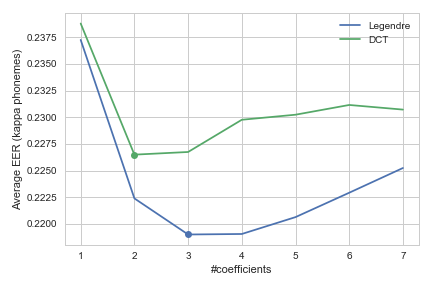
\includegraphics[width=0.5\textwidth]{files/figures/results/legendre-dct/legendre-dct-coefficients.png}
	\caption{EER average over phonemes with high Kappa as function of the number of coefficients
	for both Legendre Polynomials and DCT in the training set.}
	\label{fig:legendreVsDCT}
\end{figure}

A dot is placed on each curve showing the optimal number of coefficients for both techniques.
As it was known from \ref{fig:legendreTunning}, the optimal number of coefficients for the
Legendre Polynomials is 3 (Polynomials of degree 2). Polynomials with 4 coefficients performs
almost as well as polynomials with 3 coefficients, but it is always preferable to keep the
model as simple as possible. On the other hand, the optimal number of coefficients for DCT is 2.

The results show that when the analysis is done in isolation (in absence of the supervectors
features), Legendre Polynomials lead to a better performance, generating a relative reduction
of the average EER of 3.3\% compared with DCT.

\subsection{Comparing the Combination of Dynamic Features with Supervectors}

Even though the SVM based solely on Legendre performed better than the SVM based solely on
DCT, a new experiment is carried out in order to determine which feature integrates better
with the supervectors features to produce the best results.

Two types of combination are studied in the current thesis: a Features Combination and a Score
Combination. In the former, features from both sources are mixed in some proportion and
used to train a single SVM, and the results are obtained by running this SVM on the test data.
In the latter, an independent SVM is trained for each feature source and run against the
test data and then the results are combined in some proportion to generate the final results.

The experiment is scoped again to phonemes with high Kappa values. In this case, however, the
proportions to be used when combining the features and the scores are kept phoneme-dependent.
The objective is thus to compute for each phoneme two optimal proportions:
one for the features combinations and the other one for the score combination.

To make the experiment, proportions of the dynamic features with respect to supervectors
features were varied between 0 and 1 with steps of 0.1. In other words, the following
proportions were tested: [0.0, 0.1, 0.2 \ldots 1.0]. Both ends corresponds to use only
a feature source and not using the other source at all. A proportion of 0.0 of the dynamic
features with respect to supervectors leads to not using the dynamic features at all while
a proportion of 1.0 leads to not using the supervectors features at all.
In the case of the Features Combination, an extra exploration is done in the interval
[0.0 - 0.1], because achieving an optimal feature combination may have required a more
refined granularity in the proportions. No significant gains, however, were observed
when zooming in in the interval [0.0 - 0.1].

For the Features Combination case, the optimal proportion for the majority of the phonemes
for both Legendre and DCT approaches is 0.1. There are also some phonemes such as
$/\gamma/$ and $/b/$ where the best proprtions is 0.0. That is, that there is no
proportion of the dynamic features that produces an improvement when combined with the
supervector features.

On the other hand, for the Score Combination case, the optimal proportions for
the phonemes are more scattered along the whole interval [0.0 - 1.0] for both Legendre and
DCT. Again, there are also some phonemes where the optimal proportions is 0.0, but they are
considerable fewer than in the Features Combination case.

~

\begin{center}
    \begin{tabular}{ | c | c | c | }
    \hline
    & Legendre + Supervectors & DCT + Supervectors \\ \hline
    EER Features Combination (Avg) & 0.188 & 0.187 \\ \hline
    EER Score Combination (Avg) & 0.189  & 0.187 \\ \hline
    \end{tabular}
\end{center}

~

For both combination types, the DCT features yield better results than the Legendre features,
though the results for both features are very close to each other (around 1\% of relative
difference).

Once taken the decision of using DCT derived features to model the dynamic temporal
information, the phoneme-dependent proportions for each of the remaining phonemes with
lower Kappa values are computed for both Features Combination and Score
Combination.

\section{Main Experiment}

The final experiment is carried out to determine if there is a real gain when combining
supervectors with DCT features by testing the final models against
both the development and the heldout data.
Relative gain is calculated with respect to the baseline system: SVM trained on supervectors
features only

A McNemar test is performed as previous step to scope the analysis
to a subset of phonemes that yields statistically significant results in the development
data (\textit{p-value} $<$ 0.05).
McNemar is used to estimate confidence of the two classifiers being actually different
using the paired nominal results of both classifiers (\ref{subsection:mcnemar}).
The McNemar test is run using the SVM
trained only on supervectors as baseline of the comparison.

\subsection{Development results}

Once again, the experiment in the development set is carried out using 4-Fold Cross Validation
and taking the average of the results obtained in each fold.

Results are included only for those phonemes that were pointed out as statistically
significant for the McNemar test. Those are:

\begin{itemize}
	\item /s/, /y/, /e/, /o/, /l/, /n/, /m/ in Features Combination
	\item /s/, /y/, /e/, /o/, /l/, /z/, /n/, /m/, /rr/, /t/ in Score Combination
\end{itemize}

It is worth noting that phonemes with statistically significant gains in the Features
Combination experiment are a subset of the statistically significant phonemes in the
Score Combination experiment. For that reason, even though the barplots includes
the results for the ten statistically significant phonemes of the Score Combination,
additional marks (*) and (**) are included for the Features Combination bars to
point out whether or not those results are significant in the Features Combination
case.

\begin{figure}[H]
	\centering
	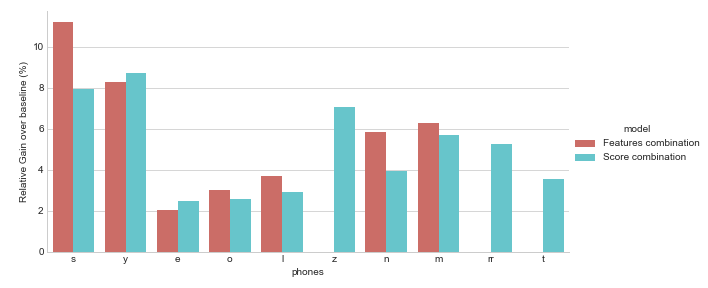
\includegraphics[width=0.8\textwidth]{files/figures/results/relatives/relatives-fusion-systems-dev-mcnemar.png}
	\caption{Comparison of performance between Features Combination system and the score combination
	of individual systems in the training set for the phones whose results were significant
	in the training set, sorted descendently by their p-value obtained in the McNemar test.
	For all the score combinations phones the results were significant in the training set,
	whereas for the features combination phones only the phones marked with (*) were significant,
	and those marked with (**) weren't significant.}
	\label{fig:fusionMcnemarDev}
\end{figure}

\subsection{Heldout results}

To run the experiment against the heldout data, the models were trained using all the
instances of the development set. A new McNemar test is performed for the results obtained
in the heldout data for the same phoneme with statistically significant results in the
development data, but this time any of them gave a significant p-value $<$ 0.05.
This can be explained by the fact that heldout data has around 1/4 of the data of the
development data, affecting the efectiveness of the test.

The results are then still scoped to the phonemes with statistically significant results
in the development experiment, and the same notation (*) and (**) is kept as a reference.

\begin{figure}[H]
	\centering
	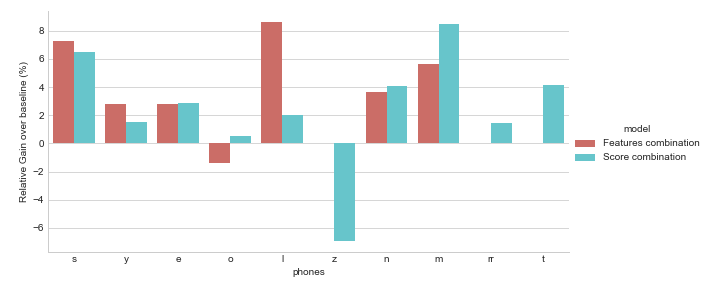
\includegraphics[width=0.8\textwidth]{files/figures/results/relatives/relative-fusion-systems-heldout-mcnemar.png}
	\caption{Comparison of performance between Features Combination system and the score combination
	of individual systems in the test set for the phones whose results were significant
	in the training set, sorted descendently by their p-value obtained in the McNemar test.
	For all the score combinations phones the results were significant in the training set,
	whereas for the features combination phones only the phones marked with (*) were significant,
	and those marked with (**) weren't significant.}
	\label{fig:fusionMcnemarTest}
\end{figure}

Among all the phonemes that were statistically significant in the Score Combination
experiment carried out in the development set, only 'z' degraded its performance compared
with the baseline system, though in a substantial way (around 6\% relative). Among the
remaining phonemes, some reduced its gain compared with the development set (such as
/y/ from 8\% to less than 2\% and /rr/ from almost 6\% to less than 2\%). Others such
as /m/ improved its performance from 6\% to more than 8\%.

On the other hand, among all the phonemes that were statistically significant in the
Features Combination experiment carried out in the development set, only /o/ degraded
its performance and in a slightly way. The plots also show a degradation of the /rr/
performance, but /rr/ is not statistically significant for the Features Combination
experiment. As in the case of the Score Combination, there are cases where both improvements
and degradations of the performance is observed.

A positive aspect of the analysis is that both /s/ and /m/, that are phonemes with high
Kappa values, yields almost the best results in both development and heldout experiments,
This fact matches the expected results and helps to
increase the confidence over the obtained results.

One important aspect to be analysed in the next section is whether or not the Score Combination
of the results leads to a more robust classifier than the Features Combination technique.


